\documentclass{article}
\usepackage[utf8]{inputenc}
\usepackage{graphicx}
\usepackage{biblatex} 
\graphicspath{ {./images/} }
\usepackage{titlesec}
\newcommand{\sectionbreak}{\clearpage} %every section on a new page


\title{Introduction to Communication Protocols}
\author{Gianluca Veschi }
\date{June 2019}

\begin{document}

\maketitle

\section{Introduction}
In the very complex world of Engineering, where many unique components within a System need to communicate with one another in order to process information and achieve a common result, it is of fundamental importance to have a consistent and robust data transmission mechanism, which guarantees that electrical signals and the bit patterns they represent are always reliably sent and received. 
\newline 
\newline     
It doesn't really matter if we are talking about a aerospace application, super computers or simply a household appliance. Electronic devices always need a communication channel, which is independent from the role in which it will be used. 
\newline 
\newline 
This paper is not going to compare different hardware systems with each other because naturally different communication interfaces have been created to be easily adapted to the individual Final system in which they will be integrated. From an abstract point of view the same concepts are valid for all the different implementations so the focus will be rather aligned with the thing that all these protocols have in common : the need to interchange information. 

\newline 
\newline 
.
\begin{figure}[h]    
    \centering
    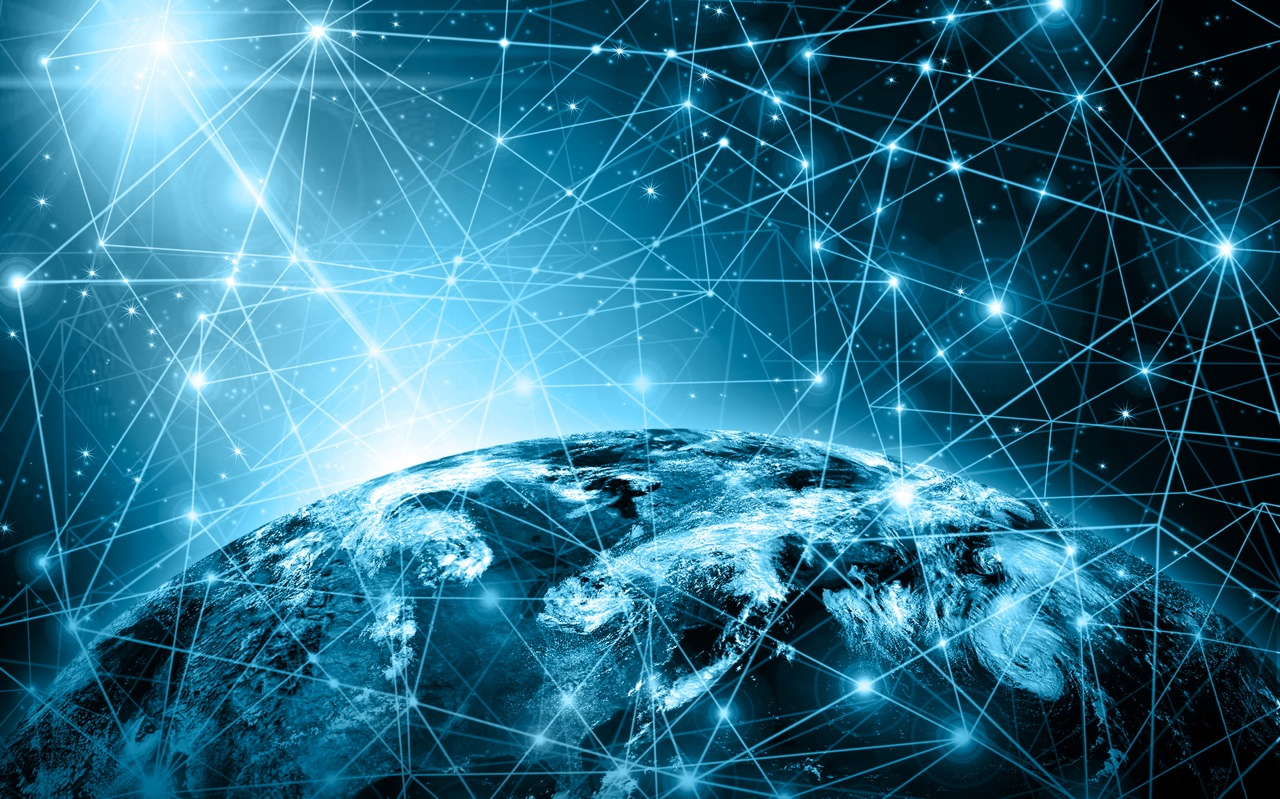
\includegraphics[width=13cm, height=6cm,center]{images/world_networks}
    \caption{World communication network}
\end{figure}


\section{Universal Serial Bus System}
The Universal Serial Bus is an industry standard protocol for communication between electronic devices, peripheral units and power supplies through cables and connectors.
\subsection{Introduction and History}
In 1994 a group of seven companies in the field of Information Technology began the development of a protocol which could allow to connect external devices to PCs in an easy way, avoiding the high number of different cables needed for each specific device with the aim of achieving a Plug'N'Play connector. The first integrated circuits supporting USB were produced by Intel in 1995 and nowadays the number of USB ports in the world is in the range of billions.
\subsection{Architecture}
The electrical structure of the USB protocol is quite complex, but it also puts the basis for a very reliable and stable communication. It became so popular because of its very high compatibility.
The system consists of a host with one or more downstream ports, to which up to 127 devices may be connected. This constraint is given by the 7 bits which can be allocated for device assignment. 
\newline
\newline
The \textbf{Host} is the organizer and master of all traffic on the bus while the devices are the so called "slaves", which communicate with the Host only when the latter has an outstanding transaction. Another important concept is the \textbf{Hub}, which expands the Host's number of available ports and also acts as a repeater.

\begin{figure}[h]    
    \centering
    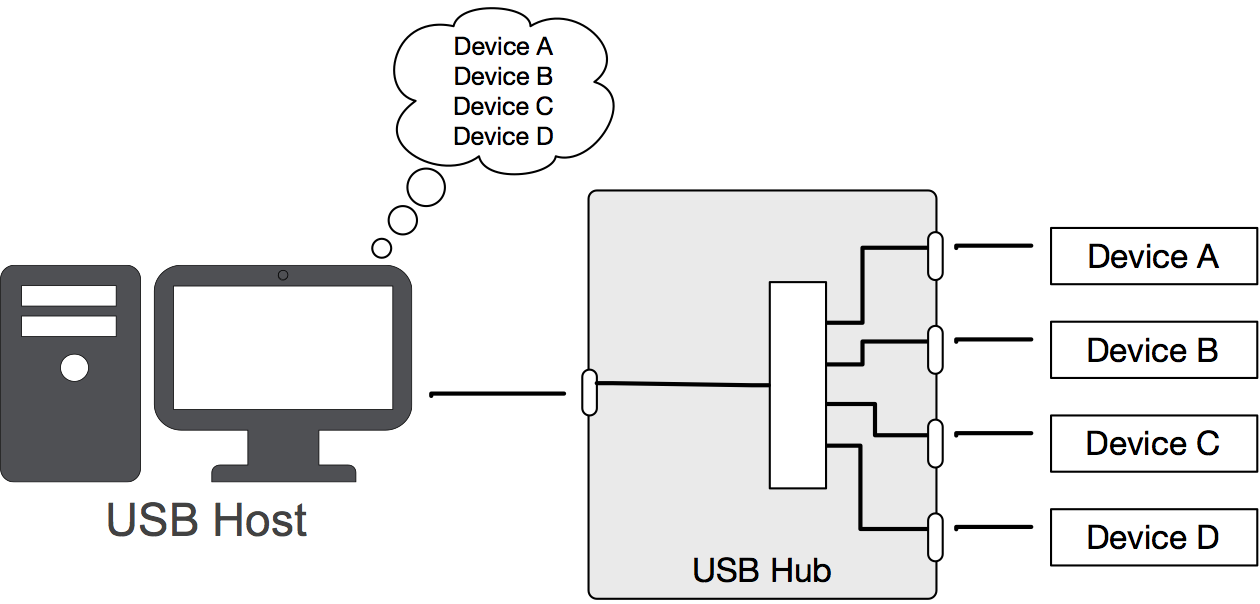
\includegraphics[width=13cm, height=6cm,center]{images/host-hub-structure}
    \caption{Host Hub Structure}
\end{figure}


The communication protocol implemented is asynchronous, which means that data is not transmitted at regular intervals, thus making variable bit rate possible. The transmitter and receiver clock generators do not have to be exactly synchronized all the time so each time a fragment of data is sent, a start bit and stop bit are needed.
\newline
\newline
The signaling makes use of the NRZI Protocol (Non Return to Zero Invert), a binary code in which ones are represented by a positive voltage and indicate a logical state change, while zeros are represented by a negative voltage and cause long period with no transition in the data. Bit stuffing is employed to ensure proper signal transitions and therefore, after six consecutive ones a zero is inserted in the data stream.
This mechanism is not self-clocking, so some additional synchronization technique is needed.

\subsubsection{Data transfer type}
There are four Transfer types which differ from each other according to the different peripherals that they will serve. Some Devices might require special attention to all the bits they send while others might be more flexible when it comes to data reliability but on the other hand would be more sensible to the speed with which their data is handled. In general the key parameters playing a role in the trade-off discussion between the different transfer types are Latency, Data Throughput and Delivery. 
    \begin{itemize}
        \item \textbf{Isochronous}\newline
            It guarantees a good latency and low data throughput but no delivery. 
            This type is intended for audio and video applications, where it's not a big deal if one bit gets lost here and there but at least it is expected to maintain the concept of time without being interrupted. The devices must be able to transfer a certain amount of data on a periodic basis and therefore failed transfers are not retried under USB, as doing so would make the connection slower and not consistent. A good Example are the video conferencing devices. 
        \item \textbf{Bulk} \newline
            It guarantees delivery but doesn't guarantee latency and has the lowest bus priority. It is used by devices such as Printers, Scanners,  Memory cards and in general anytime a transfer of large volumes of data with accuracy and no loss is expected. The transfer rate is not suited for applications that require strict management of the transfer rate because they cannot be temporarily controlled.
        \item \textbf{Interrupt} \newline
            Up to 64 bytes of data are sent per millisecond and it has the highest bus priority.
            Low Data throughput with a guaranteed latency used for Human Interface Devices which need a small amount of data which need direct attention like a mouse, a keyboard or a joystick. The input signals have to be received fast enough so that the users do not feel a "lag". The name comes from the fact that traditionally the signals where handed as interrupt requests, but given the structure of the protocol, in which only the host can initialize a data request, a inversion of control has been implemented so that the host always "polls" the input devices for new signals periodically, for example 10ms.
        \item \textbf{Control} \newline
            Unlike Interrupt, Bulk, and Isochronous transfers, Control transfers have rules about the content of the transferred data.
            Control transfers are used to exchange device details, allocate USB addresses, and configure devices, and are hence used by all devices.
        
    \end{itemize}
\subsubsection{USB Packets}
USB data transfers occur through a series of events called transactions, which are conducted within a Host-controlled time interval called frame. Something that provides the data structure for the bus and consists of multiple packets. Such a structure is always present in any Bus System even though the specific parts can differ to fit the purpose of the transmission. In the case of USB there are tree types of packets Token, Data and Handshake. 
\newline
\newline
Each transition begins with the issue of a \textbf{token} from the host. The ADDR and ENDP fields uniquely define the endpoint which must receive SETUP or OUT data.
\newline
\newline
The host issues a SOF every 1 ms. The package contains the field of the frame number which can also be used as a trigger for isochronous OUT processes.
\newline
\newline
The \textbf{Data} packets are composed of the Protocol Identifier (PID), the data field, and the CRC16 code to protect the data and finally the \textbf{Handshake} Packet containing the PID indicating the outcome of the previous communications is sent.

    
    
    \begin{figure}[h]    
    \centering
    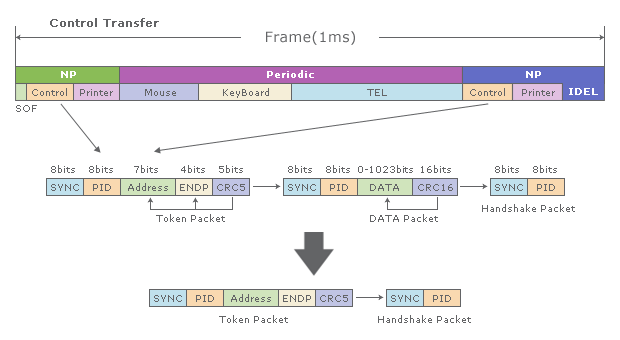
\includegraphics[width=13cm, height=6cm,center]{images/data-frame}
    \caption{data-frame}
\end{figure}

    
\subsection{Advantages}
    Given the high popularity gained by the Universal Bus System it is worth to mention the technical achievements which made this protocol so popular. It was designed to be a simple interface and this is given by multiple factors.
\begin{itemize}
    \item\textbf{ Ease of use} -  First of all there is only one single interface for multiple devices, which removes the pain of looking for hardware compatibility for different connector types. 
    \item \textbf{Auto Configuration} - The operating system of the host device only needs to install the USB device driver for once. Later whenever the peripheral device is plugged in, the driver is automatically loaded to configure the plugged in device. 
    \item \textbf{Speed} - Various speed modes are possible  which make the communication more efficient according to the type of the end device.
    \item \textbf{Reliability} - Errors are caught during data transfer so the drivers can ensure an error-free communication or also allow some errors when needed
    \item\textbf{ Low power consumption} -  No more than 500mA are needed in the worst case scenario 
    \begin{figure}[h]    
    \centering
    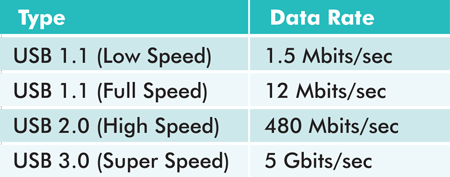
\includegraphics[width=10cm, height=4cm,center]{images/speeds-table}
    \caption{Speed Table }
    \end{figure}

    
\end{itemize}
\subsection{Limitations and Disadvantages}
\begin{itemize}
    \item Peer to Peer Communication - As per the USB standard, the communication takes place between the host and the peripheral. Two hosts cannot communicate directly to each other. Same is the case for a peripheral. On the other hand, interfaces like FireWire supports peripheral to peripheral communication. For overcoming this limitation, the USB introduced the concept of OTG (On The Go). The OTG device normally functions as peripheral, but it can also function as host with some limited capability when required. 
    \item Distance - According to USB standards, the connecting cable can be as long as 5 meters, beyond which, USB hubs need to be used for expanding the connectivity.
    \item Broadcasting -  USB does not provide the broadcasting feature, only individual messages can be communicated between host and peripheral.
    
\end{itemize}

    
    
\section{Ethernet}
\subsection{Introduction and History}
Ethernet is by far the most widely used local area networking (LAN) technology in the world today. It officialy came to life in 1973, when Bob Metcalfe described the Ethernet network system he had invented for interconnecting advanced computer workstations, making it possible to send data to one another. This led to an explosive increase in the use of information sharing applications and has brought an entire new world of communication technology into existence.

\subsection{Architecture}

In a Ethernet network the traffic of data through the cables can get pretty intense and a procedure that organizes data transmission appropriately is needed. This is done by the Carrier sense multiple access / Collision detection algorithm (CSMA/CD), which as the name says, sends data and reduces data collision. 
\newline
\newline
The operation can be compared to the behavior of a group of people who talk in a respectful way: in order for everybody to communicate properly, it is necessary that all the participants do not speak at the same time. This is done by examining the transmission medium in a polling fashion. Only when the medium remains free, a packet of data can be sent. Meanwhile the transmitter continues to examine the medium to detect collisions. 
\newline
\newline
Even though this mechanism is quite robust, collisions can still occur but they can be determined by one of the devices in the network. This is done by checking if the transmitted signal is identical to that of the transmission medium. When this is not the case it can be proved that some other device is transmitting data in the same period of time, distorting the bus signal. Inside a small LAN it is quite common to have this problem and of course the probability increases when the number of devices or the length of the transmission mediums increases.
\newline
\newline
If a collision occurs,  the module that detects it immediately interrupts the transmission and instead broadcasts an interference signal (JAM signal), which informs all the stations of the network. The station waits for a random time (Backoff) and retries the transmission. Since the two communicating devices select a random value it is unlikely that both of them attempt a transmission initialization at the same time.
\newline
\newline
The number of retransmission attempts is counted. If the following attempts continue to fail and the maximum number of attempts (16) is reached, the station notifies the upper network layer of the error and interrupts the transmission permanently, even though this is very unlikely to happen.


\subsubsection{Ethernet Frame}
The devices share data packets, also known as Ethernet packets. Among other things they contain the Ethernet frame, which is also divided into different data sets. These records consist of a binary code, which provides important information such as addresses, control information and checksums.
\newline
\newline
The size of an Ethernet frame must by default range from 64 bytes and can have a maximum of 1,518 bytes. The package always starts with a preamble that controls the synchronization between sender and receiver and a "Start Frame Delimiter" (SFD) which defines the frame. 
\newline
\newline
The information about the the destination and source addresses (MAC format) and control information in contained in the frame, which is followed by the data record to be transmitted. A "Frame Check Sequence" (FCS) closes the entire frame as checksum (except for the preamble and the SFD). The package is completed by an "Inter Frame Gap" which sets a transmission pause of 9.6 µs.
\newline
\newline
Ethernet II uses the classic frame structure, which includes the so-called "type" field, which defines various network layer protocols. In the OSI model the network layer is important for the connection and provision of network addresses. The "type" field has been replaced by a length specification in subsequent frame formats.

\begin{figure}[h]    
    \centering
    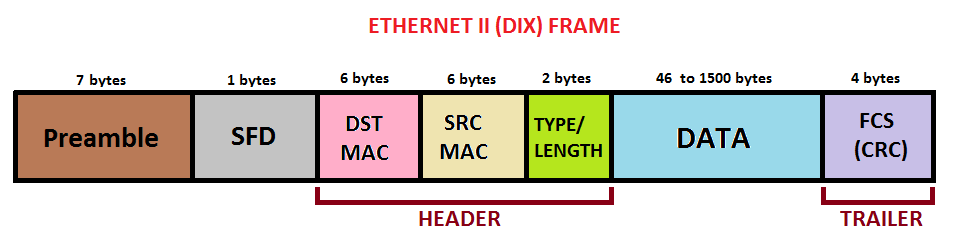
\includegraphics[width=13cm, height=4cm,center]{images/ethernet_frame}
    \caption{Ethernet II Frame}
\end{figure}



\subsubsection{Hardware Modules}
Although Ethernet is often confused with Internet they are two very different concepts and the most simple and naive explanation to somebody who doesn't have any background in technology would be that Ethernet is more of a Hardware Structure. 
There are in fact three main modules: 
\begin{itemize}
\item \textbf{Ethernet cards, or adapters} :  It is also called a "network interface card" (NIC), it's a card that plugs into a slot on the motherboard and enables a computer to access an Ethernet network (LAN). In modern computers and smartphones it usually includes a Wireless NIC, which is another adapter to interface with Wi-Fi.
\item \textbf{Ethernet cables}: This is definitely the most central part of the system and it also comes in many different forms according to the distance to which they can stretch and still carry the proper signal. This depends upon the cable's electrical transmission characteristics and is directly affected by interference around the cable. The maximum length in the case of CAT5 is for example approximately 100 meters. They look very similar to phone cables but have Eight wires which can be plugged into a Hub. These Interconnecting medias can be split up into three cathegories
\begin{itemize}
\item \textbf{Coaxial Cable} : One of the first types of interconnecting media to be used for Ethernet
\item \textbf{Twisted Pair Cables} : The two complementary signals representing the same data are sent through two cables in order to minimize the noise and thus improve the quality of the communication.
\item \textbf{Fibre Optic Cable} : This is preferred over electrical cabling when high bandwidth, long distance, or immunity to electromagnetic interference are required. It has much lower attenuation and interference and there is a large advantage in long-distances with the drawback of a complex manufacture and a expensive installation
\end{itemize}
\item \textbf{Ethernet Routers , Switches and Hubs}. These devices all work in a similar way but there are differences regarding the way they process data. The purpose of a \textbf{Hub} is to connect all of the devices together in a local network and it  doesn't provide any data filtering.  It just knows when a device is connected to one of its ports and broadcasts it to all the other ports. A \textbf{Switch} can learn the addresses of the devices connected to it and stores them in a table, so it can redirect the data to a specific target, which also helps reducing unnecessary traffic. These devices cannot exchange data outside their own local network because they don't know how to manipulate IP addresses and this is where a \textbf{Router} comes in. It can inspect the data and do all kinds of filtering and it is intended as the Gateway of the network.
\end{itemize}
\begin{figure}[h]    
    \centering
    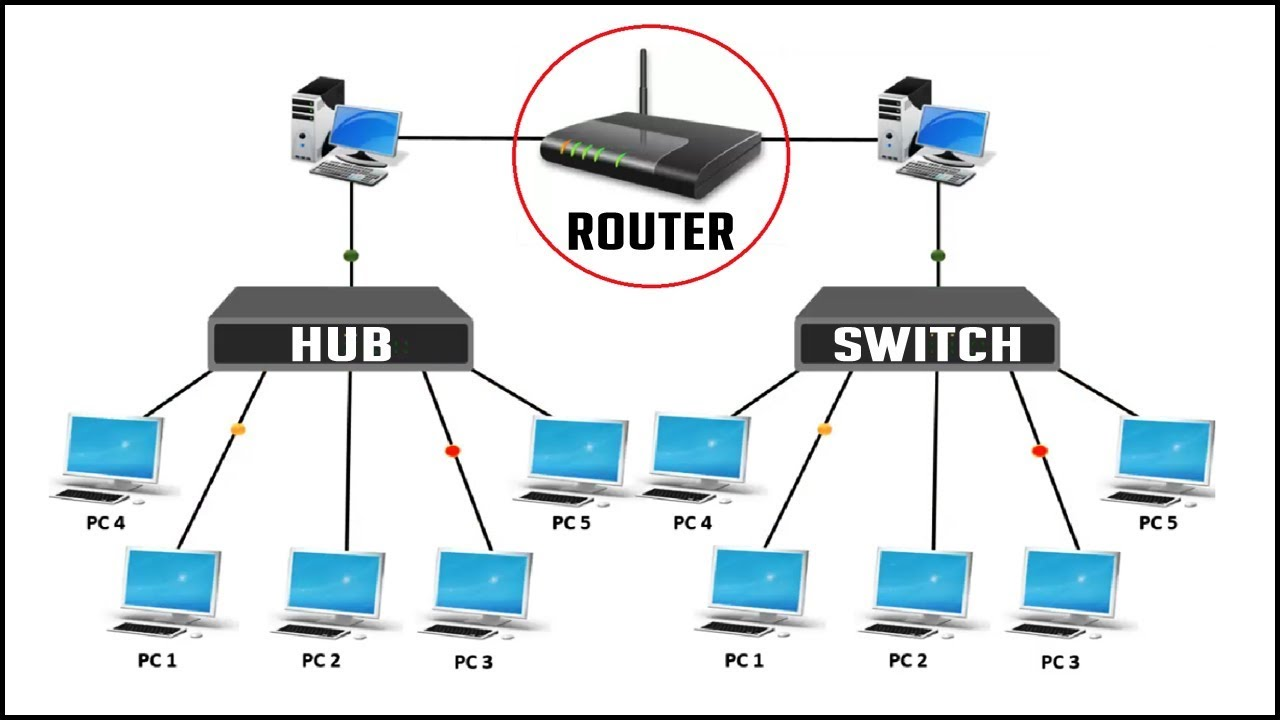
\includegraphics[width=13cm, height=6cm,center]{images/ethernet-hardware}
    \caption{Routers, Switches and Hubs}
\end{figure}
\subsubsection{Network Topologies}
The arrangement of devices in a network is a topic of high importance which pops out very often in the field of computer science.  The structure with which nodes are arranged can in fact influence the speed.
\begin{itemize}
\item \textbf{Fully Connected} : All computers and devices are connected to all other devices in the network.
\item \textbf{Star Network}   : All computers and devices are connected to a main hub or switch.
\item \textbf{Ring Network} : All computers and devices are connected to a closed loop cable without terminating ends. 
\item \textbf{Tree Network}  : All computers and devices are connected in a tree structure
\item \textbf{Bus Network}   : All computers and devices are connected to a single linear cable called trunk.
\end{itemize}

They all have their pros and cons but one of the common objectives is to have a safe network where if one devices crashes it doesn't affect all the others.
\begin{figure}[h]    
    \centering
    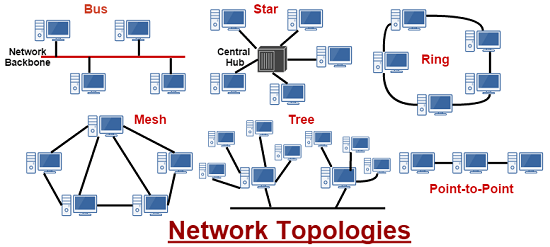
\includegraphics[width=13cm, height=6cm,center]{images/network-topologies}
    \caption{Network topologies}
\end{figure}

\subsection{Advantages}

\begin{itemize}
\item \textbf{Cost} : To form an Ethernet, not many resources and money are needed. If we do not take into account the expenses it takes to lay down fiber optic cables in the Ocean, installing hardwired networking in a office by itself is a small networking  job and presents the lowest cost option according to the estimation from an electrician or IT contractor. 
\item \textbf{Simple structure }: In Ethernet, all the nodes have the same privileges as it does not follow a  client-server architecture and consequently simplifies the administration of the system.
\item \textbf{Robustness} :  The cables used to connect systems in Ethernet are robust to noise because the used designs are usually very similar to each other and in addition to making maintenance easier the quality of the data transfer does not degrade.
\item \textbf{Speed} : Because of the many factors which affect performance there is no one specific formula that can be applied to the maximum speed rating to calculate how a connection will perform in practice but the velocity ranges from 10000 Mbps to an astonishing 100 Gbps.
\end{itemize}

\subsection{Limitations and Disadvantages}

\begin{itemize}
\item \textbf{Temperature}: Extreme temperatures could damage the Ethernet Cables and their ability to transmit signals. Cold for instance makes the cable hard to work with while elevated temperatures can degrade the plastic used in the construction. 
\item \textbf{Sensible to Noise} : When the cables are handled, the twisted pairs may open up, which could result in more cross talk or signal echoing,  factors that could cause a loss of data on the cable, resulting in process downtime or safety issues.
\item \textbf{Data Frame Size} : In Ethernet, there is a limit of the minimum size of the data field frame of 46 bytes, which has to be compensated by the Pad field in the case less data is sent. This is a disadvantage in interactive applications, where data is small and need quick transfer.
\item \textbf{No data acknowledgment method} : Ethernet is connectionless, which means that it is difficult to troubleshoot what cable or node in the network caused a problem as no acknowledge packets are sent.
\end{itemize}


 

\section{Control Area Network}
\subsection{Introduction and History}
The CAN protocol has been developed to connect Micro Controllers and other Electronics Control Units (ECU), without the need of having any central computer. It has gained momentum thanks to its many applications in the automotive world and it can also be found on trains, airplanes and other industrial systems. Not even bikes could avoid such a convenient application and examples of this protocol can in fact be found in racing models.  
\newline
\newline
We can compare a car to a human body: the vital organs fulfill one specific task and the same can be said about the modules of the system. The blood transports vital information from one organ to the other, and in the same way,  the CAN system transmits important data to the nodes of the systems in the form of electrical current through different type of cables. 
\newline
\newline
This protocol was introduced by a group of engineers working at Bosch GmbH in 1986 and it has gained so much  popularity that nowadays almost every new passenger car manufactured in Europe is equipped with at least one CAN network. Their aim was to improve the quality of automobiles by making them more reliable, safe and also fuel efficient, by creating a network of connections, where all the components can virtually be aware of what is going on in other areas. 

\begin{figure}[h]    
    \centering
    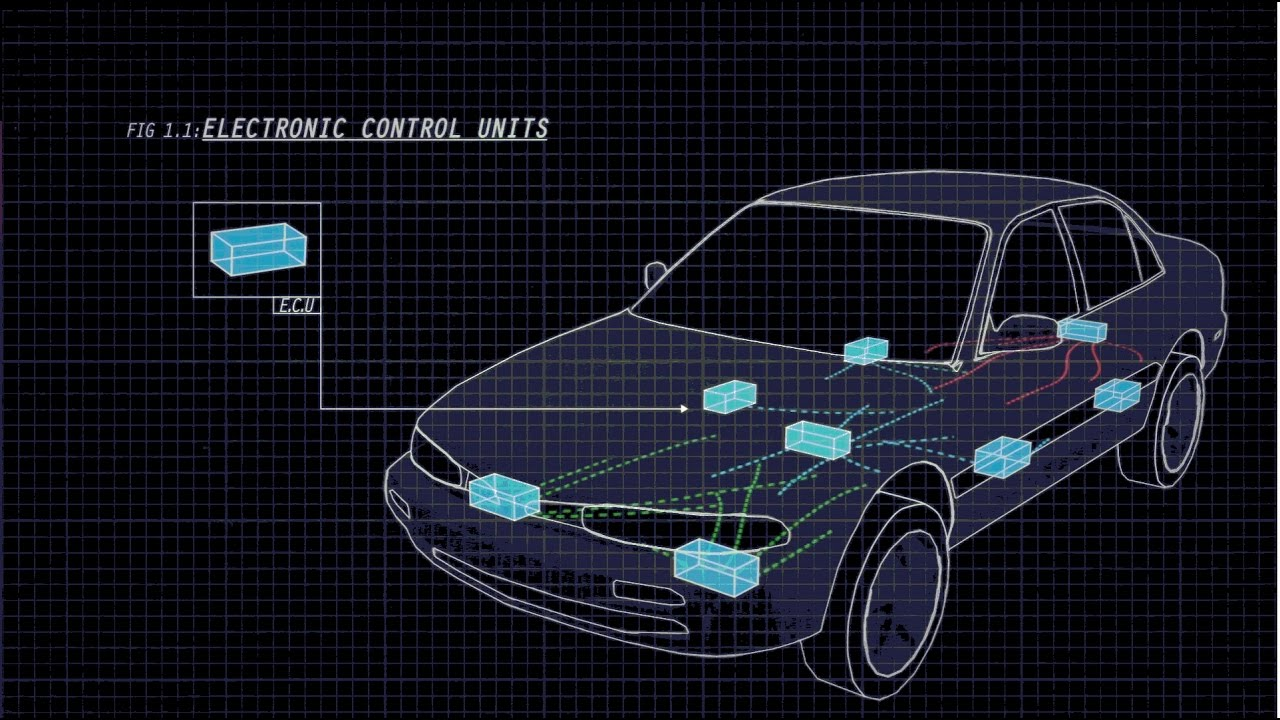
\includegraphics[width=13cm, height=8cm,center]{images/can_car}
    \caption{Example of Electronic Control Units in car}
\end{figure}


\subsection{Architecture}
CAN protocol can be defined as the set of rules for transmitting and receiving messages in a network of electronic devices and its structure consists of ECUs, which in this particular architecture are called nodes. In addition to the host controller every node has a CAN controller and CAN transceiver which are therefore responsible for sending and retrieving data over the serial bus. From a software point of view, once the two transmitting functions are written they can be easily used in each other node with little adjustments. 

\subsubsection{Physical Layer}
The physical layer of CAN, is responsible for the transfer of bits between the different nodes that make up the network. It defines aspects such as signal levels, encoding, synchronization and timing of the bits. The communication is of type broadcast, where all the ECUs are listening but react only to to the messages to which they are interested. The messages are also composed of priority levels, such that a message with low priority will not interfere with another message with a higher one.

\subsubsection{Data Link Layer}
The data link layer is responsible for media access and control
and is divided into two sub levels.
\begin{itemize}
    \item \textbf{LLC} (Logical Link Control)  : Manages the filtering of messages , flow control and error checking.
    \item \textbf{MAC} (Medium Access Control) : It is the core of the protocol. It is used for accessing the bus and the recognition of the
            messages. At the same time it can be used to to detect the status of the bus in order to start a transmission or receiving a new message. 
\end{itemize}

\begin{figure}[h]    
    \centering
    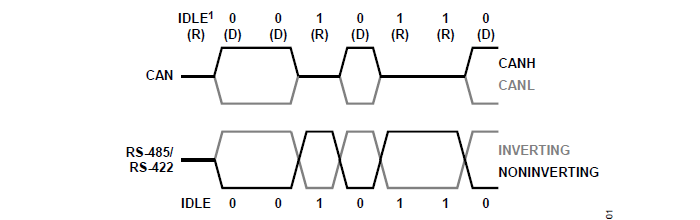
\includegraphics[width=13cm, height=4cm,center]{images/can_high_low}
    \caption{High speed CAN signaling}
\end{figure}


\newline
\newline
\subsubsection{Message Based Protocol}
CAN is a message based protocol and it does not follow the Master-Slave convention. Messages can be seen as packets which include data and other relevant information necessary for decoding. For the fact that the communication of one single ECU is broadcasted to all the other devices a identification system has been developed and there are in fact two different standards.
\begin{itemize}
    \item \textbf{Address based} : the address of the target device is written in the data.
    \item \textbf{Message based} : the message is identified by a predefined unique ID, which is usually read by the end device through a big switch statement, which acts as a filter and ignores the irrelevant messages
\end{itemize}

\subsubsection{CAN Frames}
There are different types of frames predefined by CAN for the management of the message transfer:
\begin{itemize}
    \item \textbf{Data Frame} : It is normally used to put information in the bus and is received by all nodes.
    \item \textbf{Remote Frame} : It can be used by a node to request the transmission of a data frame with the information associated with a given identifier. The receiving Node will check the authenticity of the request and provide a data frame.
    \item \textbf{Error Frame} : When a node detects an error it will abort the transmission and broadcast such a frame. After a sufficient number of errors are detected, a node will eventually turn itself off.
    \item \textbf{Overload Frame} : If a CAN node receives messages faster than it can process them then it it will send a frame to communicate the need for more time to process incoming messages.
    
\end{itemize}

In a CAN bus the nodes spontaneously transmit the information with data frames, either by a cyclical process or triggered by events in the
node. The remote interrogation frame is usually only used to detect the presence of nodes or for updating information in a newly incorporated member into the network.
\newline
\newline
In order to avoid Bus Loading the utilization should not exceed 30\% of the bus capacity to assure that low priority messages do not experience unacceptable delay. 
\newline
\newline
Messages can collide on the bus and in this case the message with the highest priority identifier will survive and the others will be retransmitted as soon as possible. This makes CAN very suitable as a real-time prioritized communications system. 

\subsubsection{Message Framing}

The Can frame consists of 8 key parts with the following roles: 

\begin{itemize}
    \item  \textbf{SOF} : Indicates the start of frame
    \item  \textbf{CAN ID}  : Identifier
    \item  \textbf{RTR} remote transmission request
    \item  \textbf{CONTROL} length in bytes
    \item  \textbf{DATA} : 64 bit data values
    \item  \textbf{CRC} cyclic redundacy check
    \item  \textbf{ACK} Acknowledgement of checksum check 
    \item  \textbf{EOF} End Of Frame
\end{itemize}

\begin{figure}[h]    
    \centering
    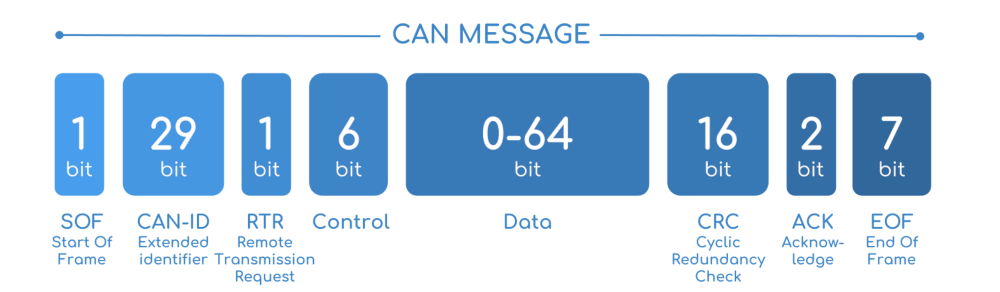
\includegraphics[width=15cm, height=4cm,center]{images/can_frame}
    \caption{CAN Frame }
\end{figure}

    



\subsection{Advantages}
\begin{itemize}
\item \textbf{Cost}: There is only one cable
\item \textbf{Broadcast capability} : Whenever a message is sent all the nodes receive it, and only the ones interested in the package know how to decode the message. This property can be very handy in case something has to be communicated to all the ECUs, such as for example the emergency situation in which the system has to shut down gracefully. 
\item \textbf{Efficiency}: Messages are prioritized via IDs so that for instance the braking system will not be interrupted by a message with a lower priority. 
\item \textbf{Robustness}: Faulty nodes don't disturb the communication so if something is broken not all the components have to be replaced. Furthermore in case of problems the CAN data logger can be used for troubleshooting.
\end{itemize}

\subsection{Limitations and Disadvantages}
The major drawback to CAN is that message latency is non-determinant (due to the existence
of Error Frames, Overload Frames and retransmissions), and latency increases with the amount of traffic on
the bus.
\newline
\newline
There is not a specified number of nodes for the network but practically it is unstable to have more than 64 as it would induce electrical loading. The maximum length supported is 40 meters and the CAN driver must produce at least 1.5V across typical 60 Ohm.


\section{Conclusion}
Although it looks like we have covered most of the topics regarding the internal communication of electronics devices for industrial and civil applications, we really just have scratched the surface of the iceberg. 
\newline
\newline
It is important to notice that there are many other protocols used in the engineering world such as the I2C, RS232 and HDLC just to mention a few. They all have their pros and cons and are mostly adapted to the roll in which they are used.
\newline
\newline
There is no solution which can embrace and realize every possible application, but fundamentally many characteristics can be considered global and are valid for any type of design. 
\newline
\newline
All communications channels basically establish a defined set of rules, to which the members have to agree in order to interface to each other. The concept of a sending and retrieving information using a defined frame is de facto always present in every implementation, no matter if we are talking about electric signals flowing through a physical media or even through the air.
\newline
\newline
Much has been accomplished since the concept of universal system bus has been created and there is still much room for improvement in speed, security and robustness.


\end{document}

